\subsection{Operating Limits and Runtime Stopping Rule}
\label{sec:eval-operating}


\begin{figure*}[!thbp]
\centering
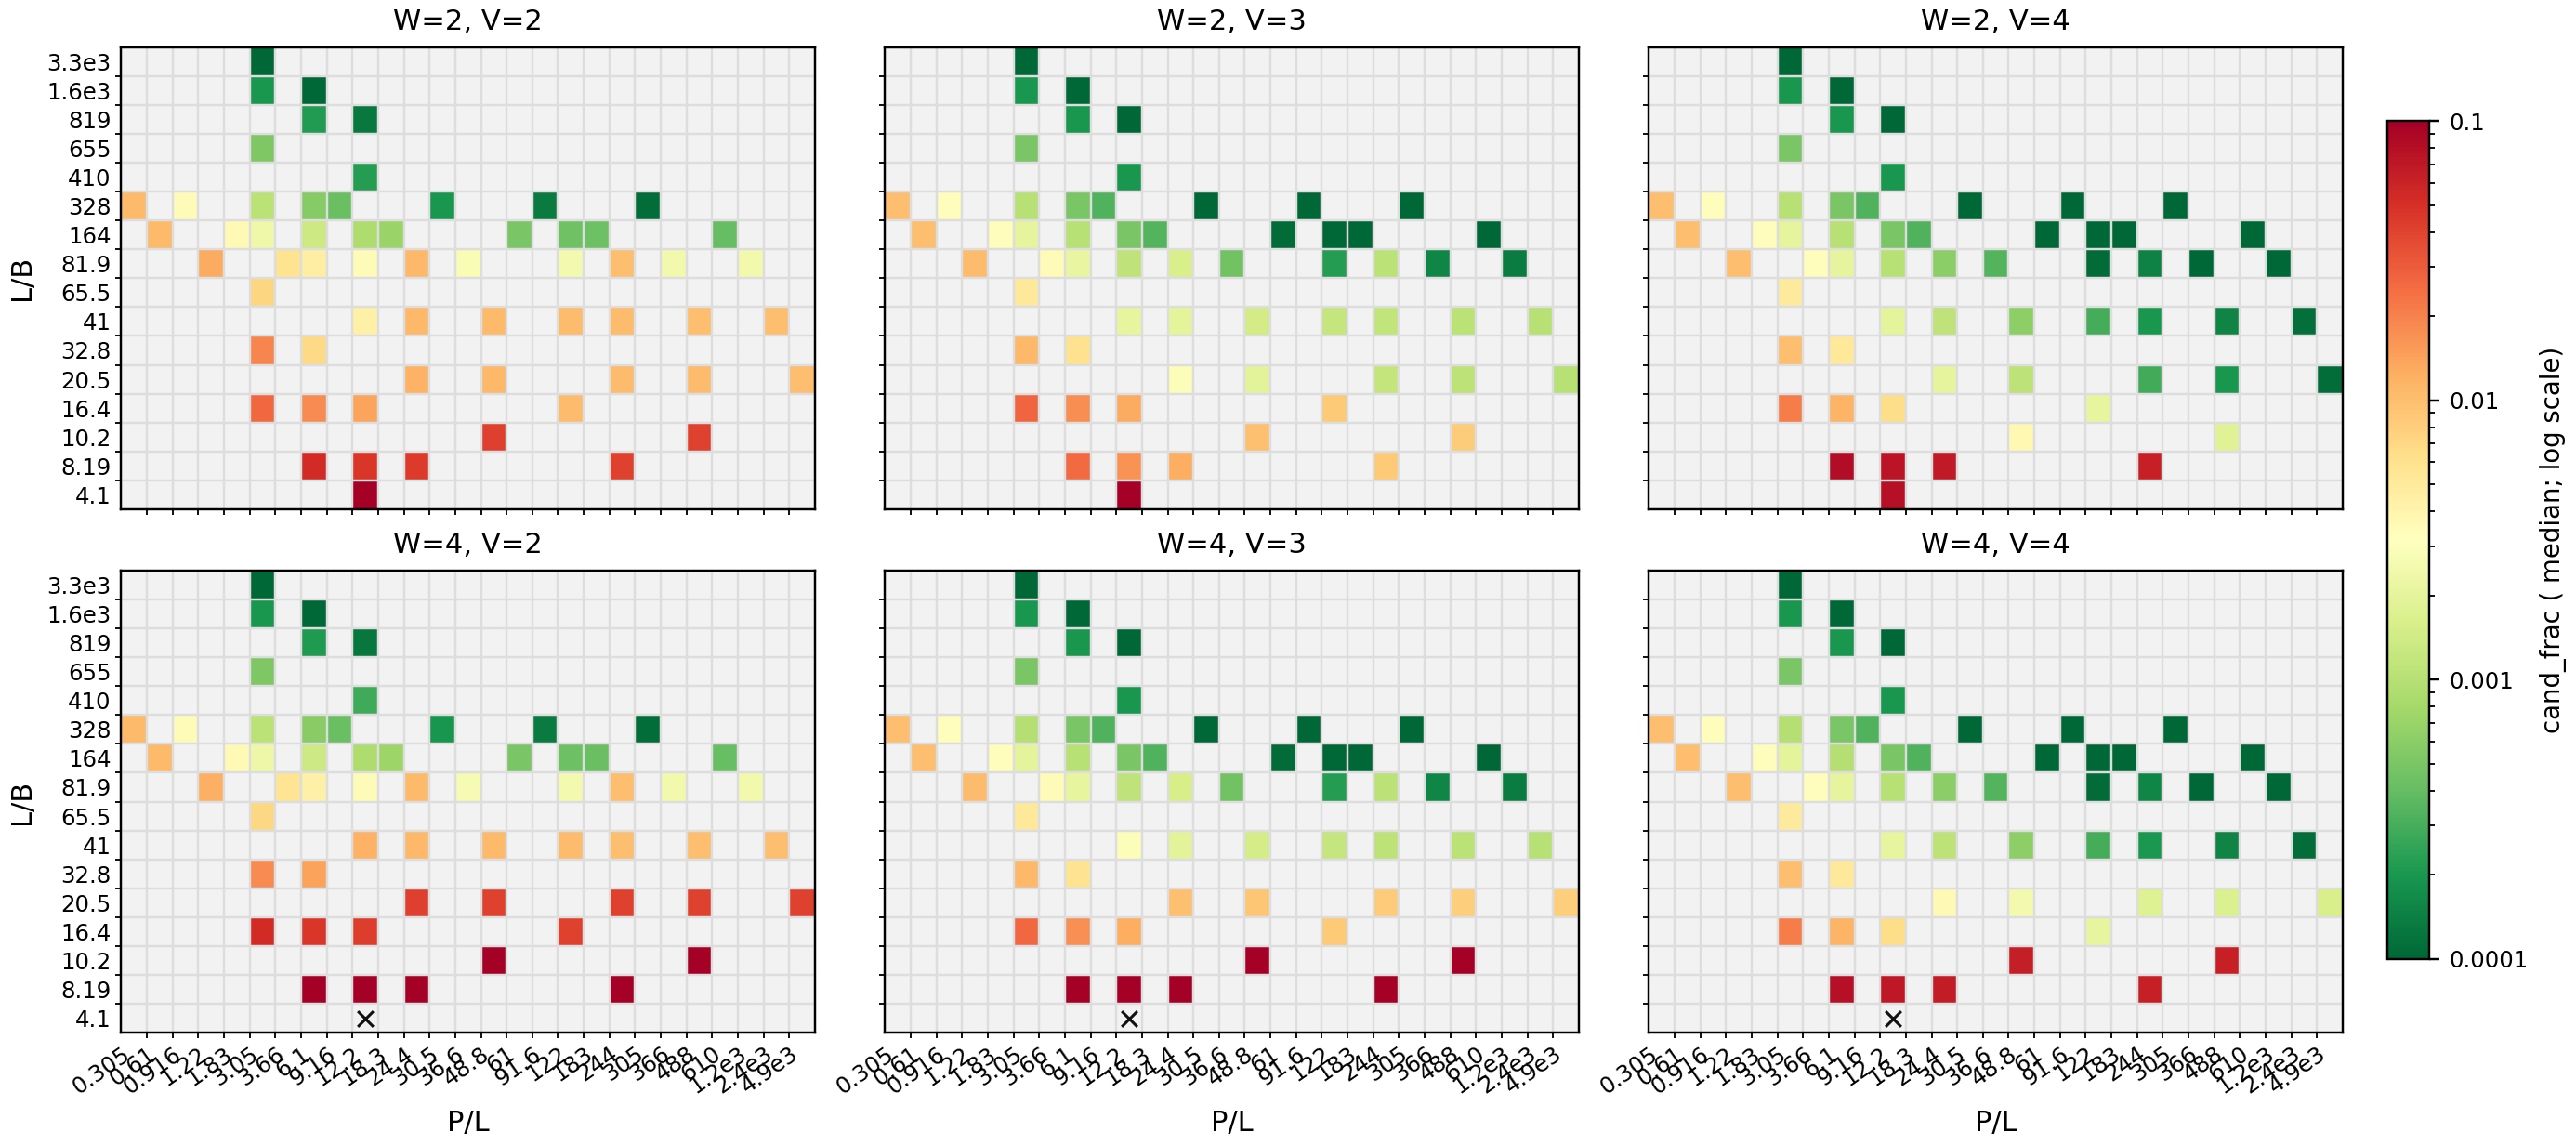
\includegraphics[width=0.93\textwidth]{figures/fig_operating_region_map_merged_heatmap.png}
 \caption{Operating region heatmap over $P/L$ and $L/B$. Color encodes the median candidate fraction \texttt{cand\_frac} on a log scale; $\times$ marks infeasible points, and gray denotes configurations with no samples.}\label{fig:c4-1}
\end{figure*}

Figure~\ref{fig:c4-1} visualizes the system's transition from effective
operation to degradation in the $(P/L,\;L/B)$ plane. The two axes govern
candidate cost through distinct mechanisms.

Along decreasing $L/B$, the $B$ dirty segments become denser on the section
axis and their high-energy windows begin to overlap, so triage must retain
more top-ranked windows to maintain recall—raising candidate cost.
Equivalently, $\texttt{cand\_frac}$ decreases monotonically with increasing
$L/B$ across all configurations. This trend is visible in the per-slice
curves of Supplement Figure~\ref{fig:c4-2}, which fix $P/L$ and sweep $L/B$.

As $P/L$ increases, the larger clean-segment pool amplifies false inclusion through the $(P-B)\,p_{\mathrm{halo}}^V$ term. 
This effect is visible even in a representative boundary slice: 
as $P/L$ grows from 1.2 to 1221,
candidate counts rise from the hundreds to the tens of thousands.
Raising $V$ from 2 to 4 reduces the count back to the hundreds,
confirming that the $P/L$-driven amplification is suppressible by
multi-view intersection (numerical details in Supplement
Table~\ref{tab:c4-1}).

Under a fixed memory budget $M_{\text{bytes}}=4VLm_0$, adding views forces $L$ to shrink proportionally ($L\propto 1/V$). More views strengthen cross-view intersection suppression exponentially, but the smaller $L$ raises the per-view halo probability $p_{\mathrm{halo}}\approx t(2W{-}1)/L$, where $t\approx \alpha BW$ and $\alpha=O(1)$ is a truncation factor. This creates a fundamental trade-off:
once $L/B$ drops below a threshold, $p_{\mathrm{halo}}$ approaches 1,
cross-view intersection loses its filtering power, and candidate cost rises
sharply. A closed-form analysis (Supplement~\ref{sec:appendix-operating-theory})
yields a sufficient condition for the intersection mechanism to remain
effective:
$
L/B \;\gtrsim\; e\alpha W(2W{-}1),
$
which evaluates to $L/B\approx 16$ for $W{=}2$, $\alpha{=}1$---the 
order of magnitude for the transition band visible in
Figure~\ref{fig:c4-1}. Above this region, the $P/L$-driven amplification
can be absorbed exponentially by multi-view intersection, and degradation
along that axis is considerably milder.


\paragraph{Runtime stopping rule}
\label{sec:eval-stoploss}
In \S\ref{sec:spatial-coupling}, triage ranks windows by energy and selects the top $t = \lceil \mathrm{r_{top}} \cdot (L-W+1) \rceil$; larger $\mathrm{r_{top}}$ yields a larger candidate set. Since $B$ is unknown at runtime and may exceed the planning prior $B^*$, SCOUT applies a runtime truncation rule.
A purely observable signal provides this adaptation. As $\mathrm{r_{top}}$ is swept upward during local decoding (a negligible in-memory computation once the probe is built), the system tracks how much energy the selected sections capture and how many candidate segments they produce.

\begin{figure}[!thbp]
\centering
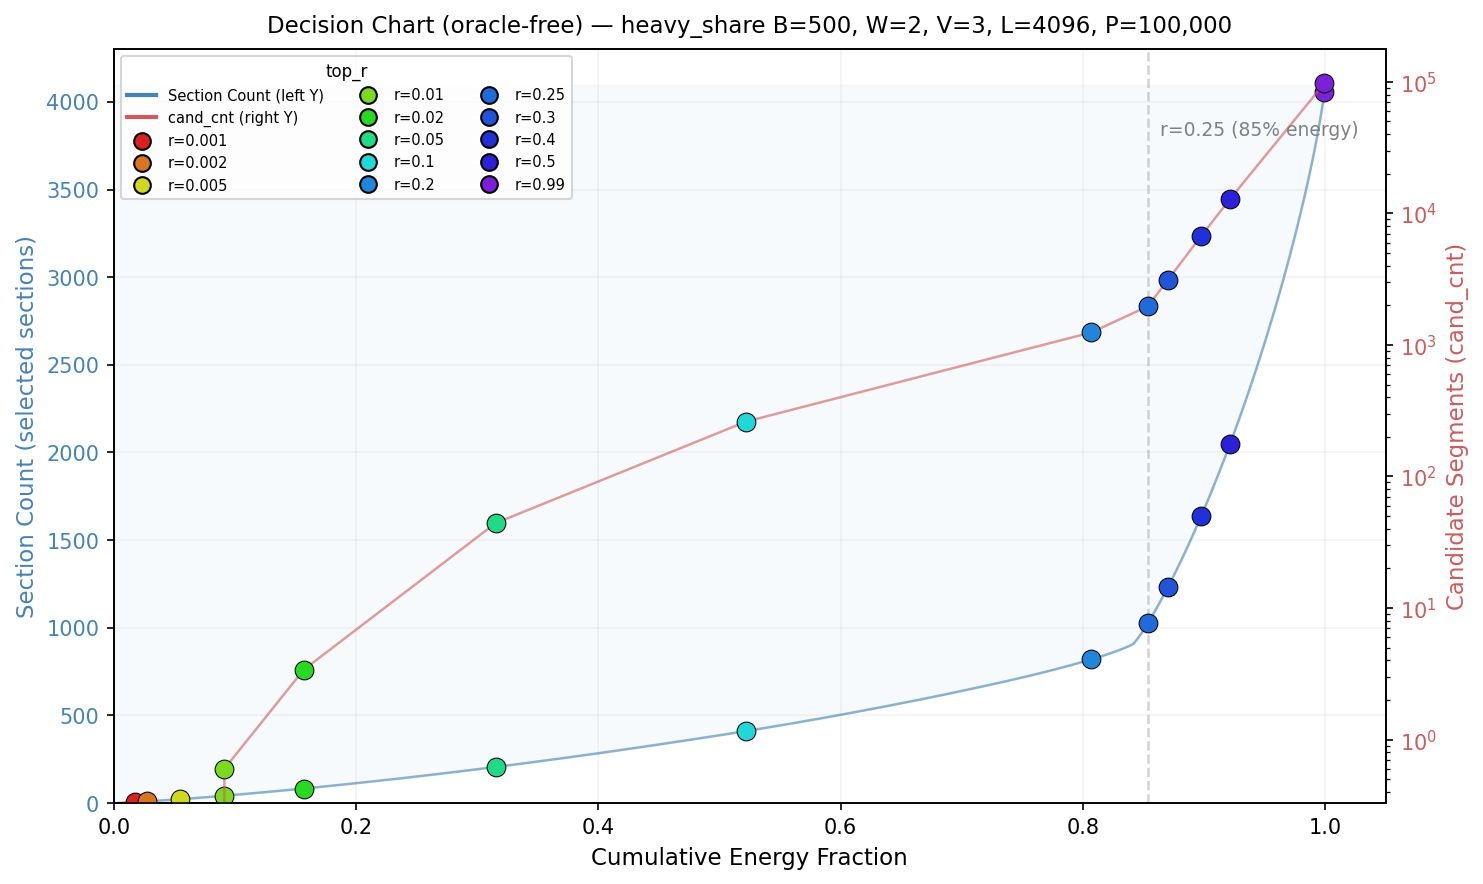
\includegraphics[width=\linewidth]{figures/decision_chart_energy_vs_cost.png}
\caption{Selected sections  (left axis) and candidate cost (right axis, log scale) plotted against cumulative energy fraction along the \texttt{top\_r} schedule. The two curves share a synchronized knee.}
\label{fig:c4-knee}
\end{figure}

Figure~\ref{fig:c4-knee} plots both quantities against cumulative energy fraction for a representative configuration. The first few top-ranked sections capture the bulk of the energy while candidate cost remains low; beyond a knee, additional sections contribute diminishing energy but candidate count accelerates sharply. This synchronized knee provides a natural stopping signal that requires no knowledge of the true~$B$: expansion halts when marginal energy gain per unit increase in candidate cost drops (implementation details in Supplement~\ref{sec:appendix-stoploss-details}). At the knee ($\mathrm{r_{top}}{=}0.25$), the cutoff captures approximately 85\% of total energy at a candidate fraction under~2\%. Doubling $\mathrm{r_{top}}$ beyond this point yields less than 5 percentage points of additional energy but increases candidate count by more than an order of magnitude.
Using ground-truth recall for offline verification, we find that this knee marks the point where additional candidate cost yields only modest recall gains (Supplement~Fig.~\ref{fig:c4-3-recall}).
